\documentclass[1p]{elsarticle_modified}
%\bibliographystyle{elsarticle-num}

%\usepackage[colorlinks]{hyperref}
%\usepackage{abbrmath_seonhwa} %\Abb, \Ascr, \Acal ,\Abf, \Afrak
\usepackage{amsfonts}
\usepackage{amssymb}
\usepackage{amsmath}
\usepackage{amsthm}
\usepackage{scalefnt}
\usepackage{amsbsy}
\usepackage{kotex}
\usepackage{caption}
\usepackage{subfig}
\usepackage{color}
\usepackage{graphicx}
\usepackage{xcolor} %% white, black, red, green, blue, cyan, magenta, yellow
\usepackage{float}
\usepackage{setspace}
\usepackage{hyperref}

\usepackage{tikz}
\usetikzlibrary{arrows}

\usepackage{multirow}
\usepackage{array} % fixed length table
\usepackage{hhline}

%%%%%%%%%%%%%%%%%%%%%
\makeatletter
\renewcommand*\env@matrix[1][\arraystretch]{%
	\edef\arraystretch{#1}%
	\hskip -\arraycolsep
	\let\@ifnextchar\new@ifnextchar
	\array{*\c@MaxMatrixCols c}}
\makeatother %https://tex.stackexchange.com/questions/14071/how-can-i-increase-the-line-spacing-in-a-matrix
%%%%%%%%%%%%%%%

\usepackage[normalem]{ulem}

\newcommand{\msout}[1]{\ifmmode\text{\sout{\ensuremath{#1}}}\else\sout{#1}\fi}
%SOURCE: \msout is \stkout macro in https://tex.stackexchange.com/questions/20609/strikeout-in-math-mode

\newcommand{\cancel}[1]{
	\ifmmode
	{\color{red}\msout{#1}}
	\else
	{\color{red}\sout{#1}}
	\fi
}

\newcommand{\add}[1]{
	{\color{blue}\uwave{#1}}
}

\newcommand{\replace}[2]{
	\ifmmode
	{\color{red}\msout{#1}}{\color{blue}\uwave{#2}}
	\else
	{\color{red}\sout{#1}}{\color{blue}\uwave{#2}}
	\fi
}

\newcommand{\Sol}{\mathcal{S}} %segment
\newcommand{\D}{D} %diagram
\newcommand{\A}{\mathcal{A}} %arc


%%%%%%%%%%%%%%%%%%%%%%%%%%%%%5 test

\def\sl{\operatorname{\textup{SL}}(2,\Cbb)}
\def\psl{\operatorname{\textup{PSL}}(2,\Cbb)}
\def\quan{\mkern 1mu \triangleright \mkern 1mu}

\theoremstyle{definition}
\newtheorem{thm}{Theorem}[section]
\newtheorem{prop}[thm]{Proposition}
\newtheorem{lem}[thm]{Lemma}
\newtheorem{ques}[thm]{Question}
\newtheorem{cor}[thm]{Corollary}
\newtheorem{defn}[thm]{Definition}
\newtheorem{exam}[thm]{Example}
\newtheorem{rmk}[thm]{Remark}
\newtheorem{alg}[thm]{Algorithm}

\newcommand{\I}{\sqrt{-1}}
\begin{document}

%\begin{frontmatter}
%
%\title{Boundary parabolic representations of knots up to 8 crossings}
%
%%% Group authors per affiliation:
%\author{Yunhi Cho} 
%\address{Department of Mathematics, University of Seoul, Seoul, Korea}
%\ead{yhcho@uos.ac.kr}
%
%
%\author{Seonhwa Kim} %\fnref{s_kim}}
%\address{Center for Geometry and Physics, Institute for Basic Science, Pohang, 37673, Korea}
%\ead{ryeona17@ibs.re.kr}
%
%\author{Hyuk Kim}
%\address{Department of Mathematical Sciences, Seoul National University, Seoul 08826, Korea}
%\ead{hyukkim@snu.ac.kr}
%
%\author{Seokbeom Yoon}
%\address{Department of Mathematical Sciences, Seoul National University, Seoul, 08826,  Korea}
%\ead{sbyoon15@snu.ac.kr}
%
%\begin{abstract}
%We find all boundary parabolic representation of knots up to 8 crossings.
%
%\end{abstract}
%\begin{keyword}
%    \MSC[2010] 57M25 
%\end{keyword}
%
%\end{frontmatter}

%\linenumbers
%\tableofcontents
%
\newcommand\colored[1]{\textcolor{white}{\rule[-0.35ex]{0.8em}{1.4ex}}\kern-0.8em\color{red} #1}%
%\newcommand\colored[1]{\textcolor{white}{ #1}\kern-2.17ex	\textcolor{white}{ #1}\kern-1.81ex	\textcolor{white}{ #1}\kern-2.15ex\color{red}#1	}

{\Large $\underline{12a_{0136}~(K12a_{0136})}$}

\setlength{\tabcolsep}{10pt}
\renewcommand{\arraystretch}{1.6}
\vspace{1cm}\begin{tabular}{m{100pt}>{\centering\arraybackslash}m{274pt}}
\multirow{5}{120pt}{
	\centering
	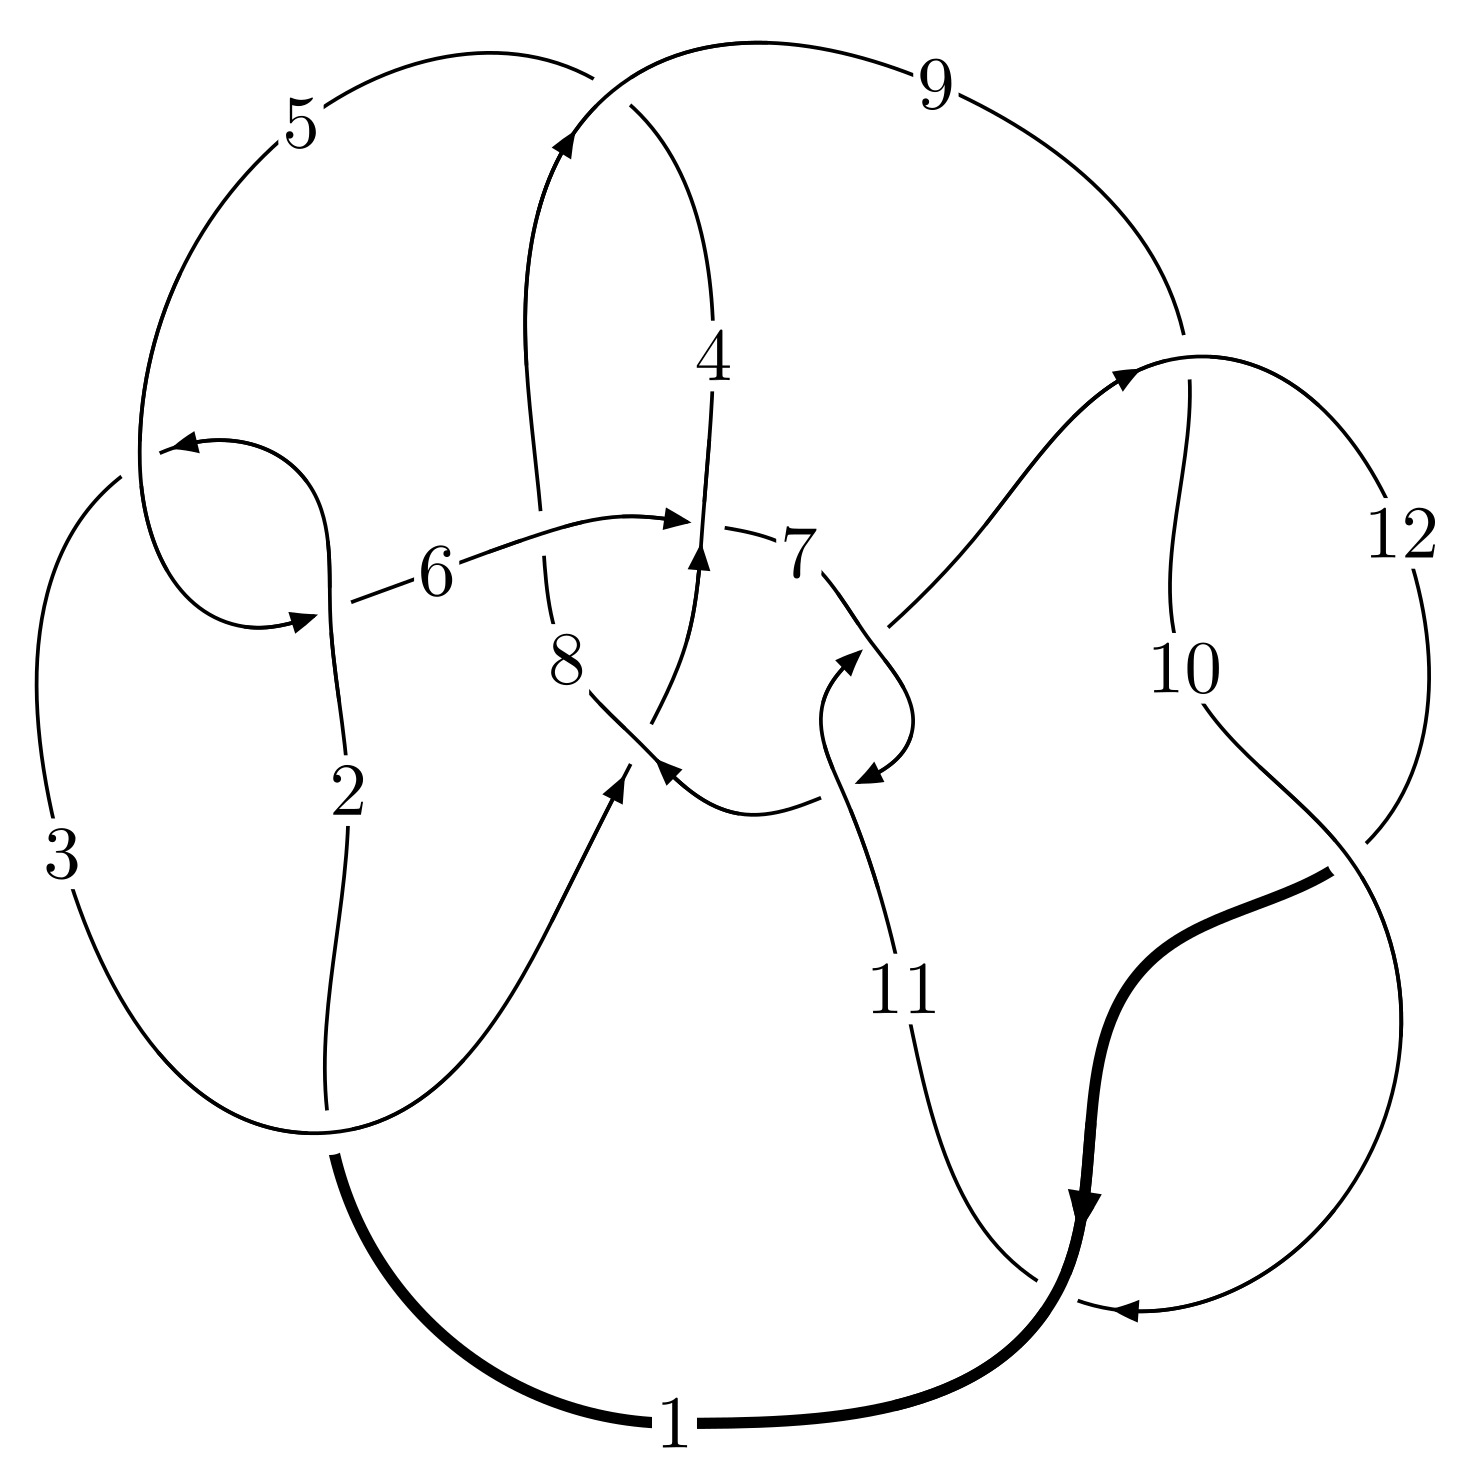
\includegraphics[width=112pt]{../../../GIT/diagram.site/Diagrams/png/937_12a_0136.png}\\
\ \ \ A knot diagram\footnotemark}&
\allowdisplaybreaks
\textbf{Linearized knot diagam} \\
\cline{2-2}
 &
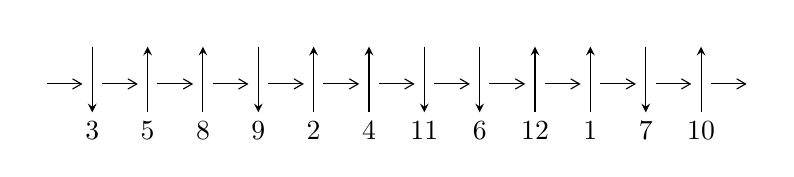
\begin{tikzpicture}[x=20pt, y=17pt]
	% nodes
	\node (C0) at (0, 0) {};
	\node (C1) at (1, 0) {};
	\node (C1U) at (1, +1) {};
	\node (C1D) at (1, -1) {3};

	\node (C2) at (2, 0) {};
	\node (C2U) at (2, +1) {};
	\node (C2D) at (2, -1) {5};

	\node (C3) at (3, 0) {};
	\node (C3U) at (3, +1) {};
	\node (C3D) at (3, -1) {8};

	\node (C4) at (4, 0) {};
	\node (C4U) at (4, +1) {};
	\node (C4D) at (4, -1) {9};

	\node (C5) at (5, 0) {};
	\node (C5U) at (5, +1) {};
	\node (C5D) at (5, -1) {2};

	\node (C6) at (6, 0) {};
	\node (C6U) at (6, +1) {};
	\node (C6D) at (6, -1) {4};

	\node (C7) at (7, 0) {};
	\node (C7U) at (7, +1) {};
	\node (C7D) at (7, -1) {11};

	\node (C8) at (8, 0) {};
	\node (C8U) at (8, +1) {};
	\node (C8D) at (8, -1) {6};

	\node (C9) at (9, 0) {};
	\node (C9U) at (9, +1) {};
	\node (C9D) at (9, -1) {12};

	\node (C10) at (10, 0) {};
	\node (C10U) at (10, +1) {};
	\node (C10D) at (10, -1) {1};

	\node (C11) at (11, 0) {};
	\node (C11U) at (11, +1) {};
	\node (C11D) at (11, -1) {7};

	\node (C12) at (12, 0) {};
	\node (C12U) at (12, +1) {};
	\node (C12D) at (12, -1) {10};
	\node (C13) at (13, 0) {};

	% arrows
	\draw[->,>={angle 60}]
	(C0) edge (C1) (C1) edge (C2) (C2) edge (C3) (C3) edge (C4) (C4) edge (C5) (C5) edge (C6) (C6) edge (C7) (C7) edge (C8) (C8) edge (C9) (C9) edge (C10) (C10) edge (C11) (C11) edge (C12) (C12) edge (C13) ;	\draw[->,>=stealth]
	(C1U) edge (C1D) (C2D) edge (C2U) (C3D) edge (C3U) (C4U) edge (C4D) (C5D) edge (C5U) (C6D) edge (C6U) (C7U) edge (C7D) (C8U) edge (C8D) (C9D) edge (C9U) (C10D) edge (C10U) (C11U) edge (C11D) (C12D) edge (C12U) ;
	\end{tikzpicture} \\
\hhline{~~} \\& 
\textbf{Solving Sequence} \\ \cline{2-2} 
 &
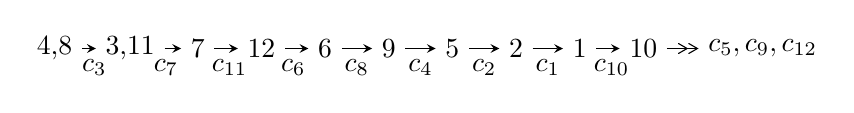
\begin{tikzpicture}[x=23pt, y=7pt]
	% node
	\node (A0) at (-1/8, 0) {4,8};
	\node (A1) at (17/16, 0) {3,11};
	\node (A2) at (17/8, 0) {7};
	\node (A3) at (25/8, 0) {12};
	\node (A4) at (33/8, 0) {6};
	\node (A5) at (41/8, 0) {9};
	\node (A6) at (49/8, 0) {5};
	\node (A7) at (57/8, 0) {2};
	\node (A8) at (65/8, 0) {1};
	\node (A9) at (73/8, 0) {10};
	\node (C1) at (1/2, -1) {$c_{3}$};
	\node (C2) at (13/8, -1) {$c_{7}$};
	\node (C3) at (21/8, -1) {$c_{11}$};
	\node (C4) at (29/8, -1) {$c_{6}$};
	\node (C5) at (37/8, -1) {$c_{8}$};
	\node (C6) at (45/8, -1) {$c_{4}$};
	\node (C7) at (53/8, -1) {$c_{2}$};
	\node (C8) at (61/8, -1) {$c_{1}$};
	\node (C9) at (69/8, -1) {$c_{10}$};
	\node (A10) at (11, 0) {$c_{5},c_{9},c_{12}$};

	% edge
	\draw[->,>=stealth]	
	(A0) edge (A1) (A1) edge (A2) (A2) edge (A3) (A3) edge (A4) (A4) edge (A5) (A5) edge (A6) (A6) edge (A7) (A7) edge (A8) (A8) edge (A9) ;
	\draw[->>,>={angle 60}]	
	(A9) edge (A10);
\end{tikzpicture} \\ 

\end{tabular} \\

\footnotetext{
The image of knot diagram is generated by the software ``\textbf{Draw programme}" developed by Andrew Bartholomew(\url{http://www.layer8.co.uk/maths/draw/index.htm\#Running-draw}), where we modified some parts for our purpose(\url{https://github.com/CATsTAILs/LinksPainter}).
}\phantom \\ \newline 
\centering \textbf{Ideals for irreducible components\footnotemark of $X_{\text{par}}$} 
 
\begin{align*}
I^u_{1}&=\langle 
1.92138\times10^{1091} u^{118}+4.64324\times10^{1091} u^{117}+\cdots+1.00650\times10^{1094} b+1.39253\times10^{1096},\\
\phantom{I^u_{1}}&\phantom{= \langle  }-1.61183\times10^{1095} u^{118}-4.22365\times10^{1095} u^{117}+\cdots+3.08521\times10^{1098} a-6.78233\times10^{1099},\\
\phantom{I^u_{1}}&\phantom{= \langle  }u^{119}+2 u^{118}+\cdots+83530 u-30653\rangle \\
I^u_{2}&=\langle 
- u^2+b+u-1,\;a,\;u^4+u^2+u+1\rangle \\
I^u_{3}&=\langle 
2 u^5+3 u^3- u^2+b+2 u-2,\;a,\;u^6- u^5+2 u^4-2 u^3+2 u^2-2 u+1\rangle \\
\\
\end{align*}
\raggedright * 3 irreducible components of $\dim_{\mathbb{C}}=0$, with total 129 representations.\\
\footnotetext{All coefficients of polynomials are rational numbers. But the coefficients are sometimes approximated in decimal forms when there is not enough margin.}
\newpage
\renewcommand{\arraystretch}{1}
\centering \section*{I. $I^u_{1}= \langle 1.92\times10^{1091} u^{118}+4.64\times10^{1091} u^{117}+\cdots+1.01\times10^{1094} b+1.39\times10^{1096},\;-1.61\times10^{1095} u^{118}-4.22\times10^{1095} u^{117}+\cdots+3.09\times10^{1098} a-6.78\times10^{1099},\;u^{119}+2 u^{118}+\cdots+83530 u-30653 \rangle$}
\flushleft \textbf{(i) Arc colorings}\\
\begin{tabular}{m{7pt} m{180pt} m{7pt} m{180pt} }
\flushright $a_{4}=$&$\begin{pmatrix}1\\0\end{pmatrix}$ \\
\flushright $a_{8}=$&$\begin{pmatrix}0\\u\end{pmatrix}$ \\
\flushright $a_{3}=$&$\begin{pmatrix}1\\u^2\end{pmatrix}$ \\
\flushright $a_{11}=$&$\begin{pmatrix}0.000522436 u^{118}+0.00136900 u^{117}+\cdots+6.20057 u+21.9834\\-0.00190898 u^{118}-0.00461328 u^{117}+\cdots+48.5697 u-138.354\end{pmatrix}$ \\
\flushright $a_{7}=$&$\begin{pmatrix}-0.00200655 u^{118}-0.00486829 u^{117}+\cdots+55.9628 u-133.379\\-0.00152654 u^{118}-0.00376370 u^{117}+\cdots+65.0969 u-99.4643\end{pmatrix}$ \\
\flushright $a_{12}=$&$\begin{pmatrix}-0.00285140 u^{118}-0.00709019 u^{117}+\cdots+151.015 u-185.338\\-0.00192121 u^{118}-0.00470284 u^{117}+\cdots+64.2476 u-130.571\end{pmatrix}$ \\
\flushright $a_{6}=$&$\begin{pmatrix}-0.000480013 u^{118}-0.00110460 u^{117}+\cdots-9.13415 u-33.9147\\-0.00152654 u^{118}-0.00376370 u^{117}+\cdots+65.0969 u-99.4643\end{pmatrix}$ \\
\flushright $a_{9}=$&$\begin{pmatrix}0.00245573 u^{118}+0.00629867 u^{117}+\cdots-225.013 u+121.139\\-0.00168112 u^{118}-0.00408093 u^{117}+\cdots+55.9312 u-118.865\end{pmatrix}$ \\
\flushright $a_{5}=$&$\begin{pmatrix}-0.00412868 u^{118}-0.0102821 u^{117}+\cdots+131.372 u-247.767\\-0.00103999 u^{118}-0.00252566 u^{117}+\cdots+35.1546 u-74.9025\end{pmatrix}$ \\
\flushright $a_{2}=$&$\begin{pmatrix}-0.00467142 u^{118}-0.0112071 u^{117}+\cdots+116.802 u-339.632\\0.00104931 u^{118}+0.00255345 u^{117}+\cdots-31.3528 u+73.5724\end{pmatrix}$ \\
\flushright $a_{1}=$&$\begin{pmatrix}-0.00289772 u^{118}-0.00693478 u^{117}+\cdots+72.9161 u-208.913\\0.00133844 u^{118}+0.00324465 u^{117}+\cdots-37.5398 u+95.7947\end{pmatrix}$ \\
\flushright $a_{10}=$&$\begin{pmatrix}-0.00225121 u^{118}-0.00540515 u^{117}+\cdots+56.8808 u-167.552\\-0.00193168 u^{118}-0.00471512 u^{117}+\cdots+65.4873 u-133.140\end{pmatrix}$\\&\end{tabular}
\flushleft \textbf{(ii) Obstruction class $= -1$}\\~\\
\flushleft \textbf{(iii) Cusp Shapes $= 0.00773579 u^{118}+0.0192693 u^{117}+\cdots-357.195 u+464.026$}\\~\\
\newpage\renewcommand{\arraystretch}{1}
\flushleft \textbf{(iv) u-Polynomials at the component}\newline \\
\begin{tabular}{m{50pt}|m{274pt}}
Crossings & \hspace{64pt}u-Polynomials at each crossing \\
\hline $$\begin{aligned}c_{1}\end{aligned}$$&$\begin{aligned}
&u^{119}+48 u^{118}+\cdots+10 u-1
\end{aligned}$\\
\hline $$\begin{aligned}c_{2},c_{5}\end{aligned}$$&$\begin{aligned}
&u^{119}+2 u^{118}+\cdots+10 u-1
\end{aligned}$\\
\hline $$\begin{aligned}c_{3}\end{aligned}$$&$\begin{aligned}
&u^{119}-2 u^{118}+\cdots+83530 u+30653
\end{aligned}$\\
\hline $$\begin{aligned}c_{4}\end{aligned}$$&$\begin{aligned}
&u^{119}+2 u^{118}+\cdots-140120 u+18392
\end{aligned}$\\
\hline $$\begin{aligned}c_{6}\end{aligned}$$&$\begin{aligned}
&u^{119}+12 u^{118}+\cdots+2 u+1
\end{aligned}$\\
\hline $$\begin{aligned}c_{7},c_{11}\end{aligned}$$&$\begin{aligned}
&u^{119}+u^{118}+\cdots+8192 u-1024
\end{aligned}$\\
\hline $$\begin{aligned}c_{8}\end{aligned}$$&$\begin{aligned}
&u^{119}-10 u^{118}+\cdots-2 u+1
\end{aligned}$\\
\hline $$\begin{aligned}c_{9},c_{10},c_{12}\end{aligned}$$&$\begin{aligned}
&u^{119}+11 u^{118}+\cdots-5 u-1
\end{aligned}$\\
\hline
\end{tabular}\\~\\
\newpage\renewcommand{\arraystretch}{1}
\flushleft \textbf{(v) Riley Polynomials at the component}\newline \\
\begin{tabular}{m{50pt}|m{274pt}}
Crossings & \hspace{64pt}Riley Polynomials at each crossing \\
\hline $$\begin{aligned}c_{1}\end{aligned}$$&$\begin{aligned}
&y^{119}+48 y^{118}+\cdots+2322 y-1
\end{aligned}$\\
\hline $$\begin{aligned}c_{2},c_{5}\end{aligned}$$&$\begin{aligned}
&y^{119}+48 y^{118}+\cdots+10 y-1
\end{aligned}$\\
\hline $$\begin{aligned}c_{3}\end{aligned}$$&$\begin{aligned}
&y^{119}+108 y^{118}+\cdots-59171729182 y-939606409
\end{aligned}$\\
\hline $$\begin{aligned}c_{4}\end{aligned}$$&$\begin{aligned}
&y^{119}+132 y^{118}+\cdots-23236923728 y-338265664
\end{aligned}$\\
\hline $$\begin{aligned}c_{6}\end{aligned}$$&$\begin{aligned}
&y^{119}+120 y^{117}+\cdots+10 y-1
\end{aligned}$\\
\hline $$\begin{aligned}c_{7},c_{11}\end{aligned}$$&$\begin{aligned}
&y^{119}+63 y^{118}+\cdots-16252928 y-1048576
\end{aligned}$\\
\hline $$\begin{aligned}c_{8}\end{aligned}$$&$\begin{aligned}
&y^{119}+12 y^{118}+\cdots-10 y-1
\end{aligned}$\\
\hline $$\begin{aligned}c_{9},c_{10},c_{12}\end{aligned}$$&$\begin{aligned}
&y^{119}-111 y^{118}+\cdots+61 y-1
\end{aligned}$\\
\hline
\end{tabular}\\~\\
\newpage\flushleft \textbf{(vi) Complex Volumes and Cusp Shapes}
$$\begin{array}{c|c|c}  
\text{Solutions to }I^u_{1}& \I (\text{vol} + \sqrt{-1}CS) & \text{Cusp shape}\\
 \hline 
\begin{aligned}
u &= \phantom{-}0.227226 + 0.970712 I \\
a &= -0.069245 + 0.726320 I \\
b &= -0.003345 + 0.144442 I\end{aligned}
 & -3.66803 - 0.76142 I & \phantom{-0.000000 } 0 \\ \hline\begin{aligned}
u &= \phantom{-}0.227226 - 0.970712 I \\
a &= -0.069245 - 0.726320 I \\
b &= -0.003345 - 0.144442 I\end{aligned}
 & -3.66803 + 0.76142 I & \phantom{-0.000000 } 0 \\ \hline\begin{aligned}
u &= -0.458534 + 0.875185 I \\
a &= -0.573576 + 0.749123 I \\
b &= \phantom{-}1.05671 + 2.08096 I\end{aligned}
 & -1.51868 - 2.01224 I & \phantom{-0.000000 } 0 \\ \hline\begin{aligned}
u &= -0.458534 - 0.875185 I \\
a &= -0.573576 - 0.749123 I \\
b &= \phantom{-}1.05671 - 2.08096 I\end{aligned}
 & -1.51868 + 2.01224 I & \phantom{-0.000000 } 0 \\ \hline\begin{aligned}
u &= -0.871485 + 0.537431 I \\
a &= -0.266119 + 0.944276 I \\
b &= \phantom{-}0.39942 + 1.42963 I\end{aligned}
 & \phantom{-}0.69537 - 1.96234 I & \phantom{-0.000000 } 0 \\ \hline\begin{aligned}
u &= -0.871485 - 0.537431 I \\
a &= -0.266119 - 0.944276 I \\
b &= \phantom{-}0.39942 - 1.42963 I\end{aligned}
 & \phantom{-}0.69537 + 1.96234 I & \phantom{-0.000000 } 0 \\ \hline\begin{aligned}
u &= \phantom{-}0.570079 + 0.787703 I \\
a &= -0.943640 + 0.550499 I \\
b &= -0.518404 + 0.107984 I\end{aligned}
 & -0.70650 + 4.43937 I & \phantom{-0.000000 } 0 \\ \hline\begin{aligned}
u &= \phantom{-}0.570079 - 0.787703 I \\
a &= -0.943640 - 0.550499 I \\
b &= -0.518404 - 0.107984 I\end{aligned}
 & -0.70650 - 4.43937 I & \phantom{-0.000000 } 0 \\ \hline\begin{aligned}
u &= -0.843856 + 0.434969 I \\
a &= -0.490567 + 0.773091 I \\
b &= -0.74992 + 1.76092 I\end{aligned}
 & \phantom{-}2.05334 - 2.32542 I & \phantom{-0.000000 } 0 \\ \hline\begin{aligned}
u &= -0.843856 - 0.434969 I \\
a &= -0.490567 - 0.773091 I \\
b &= -0.74992 - 1.76092 I\end{aligned}
 & \phantom{-}2.05334 + 2.32542 I & \phantom{-0.000000 } 0\\
 \hline 
 \end{array}$$\newpage$$\begin{array}{c|c|c}  
\text{Solutions to }I^u_{1}& \I (\text{vol} + \sqrt{-1}CS) & \text{Cusp shape}\\
 \hline 
\begin{aligned}
u &= \phantom{-}0.578503 + 0.878040 I \\
a &= -0.63889 - 1.34499 I \\
b &= \phantom{-}0.393897 - 1.228490 I\end{aligned}
 & \phantom{-}6.53771 + 10.99580 I & \phantom{-0.000000 } 0 \\ \hline\begin{aligned}
u &= \phantom{-}0.578503 - 0.878040 I \\
a &= -0.63889 + 1.34499 I \\
b &= \phantom{-}0.393897 + 1.228490 I\end{aligned}
 & \phantom{-}6.53771 - 10.99580 I & \phantom{-0.000000 } 0 \\ \hline\begin{aligned}
u &= \phantom{-}0.647414 + 0.685423 I \\
a &= -0.426111 - 0.105610 I \\
b &= \phantom{-}1.25322 + 0.74492 I\end{aligned}
 & -0.42288 - 2.75298 I & \phantom{-0.000000 } 0 \\ \hline\begin{aligned}
u &= \phantom{-}0.647414 - 0.685423 I \\
a &= -0.426111 + 0.105610 I \\
b &= \phantom{-}1.25322 - 0.74492 I\end{aligned}
 & -0.42288 + 2.75298 I & \phantom{-0.000000 } 0 \\ \hline\begin{aligned}
u &= -0.682886 + 0.836097 I \\
a &= \phantom{-}0.412953 - 0.990140 I \\
b &= -0.70679 - 2.20076 I\end{aligned}
 & -3.60584 - 6.39853 I & \phantom{-0.000000 } 0 \\ \hline\begin{aligned}
u &= -0.682886 - 0.836097 I \\
a &= \phantom{-}0.412953 + 0.990140 I \\
b &= -0.70679 + 2.20076 I\end{aligned}
 & -3.60584 + 6.39853 I & \phantom{-0.000000 } 0 \\ \hline\begin{aligned}
u &= \phantom{-}0.905424 + 0.062884 I \\
a &= \phantom{-}0.220350 - 1.122690 I \\
b &= \phantom{-}0.82535 - 2.10816 I\end{aligned}
 & \phantom{-}3.36143 + 3.82787 I & \phantom{-0.000000 } 0 \\ \hline\begin{aligned}
u &= \phantom{-}0.905424 - 0.062884 I \\
a &= \phantom{-}0.220350 + 1.122690 I \\
b &= \phantom{-}0.82535 + 2.10816 I\end{aligned}
 & \phantom{-}3.36143 - 3.82787 I & \phantom{-0.000000 } 0 \\ \hline\begin{aligned}
u &= \phantom{-}0.891680\phantom{ +0.000000I} \\
a &= \phantom{-}1.06076\phantom{ +0.000000I} \\
b &= -0.552916\phantom{ +0.000000I}\end{aligned}
 & \phantom{-}2.76788\phantom{ +0.000000I} & \phantom{-0.000000 } 0 \\ \hline\begin{aligned}
u &= -0.412585 + 0.786762 I \\
a &= -0.97982 + 1.20779 I \\
b &= -0.96051 + 1.16770 I\end{aligned}
 & \phantom{-}7.05259 - 9.90887 I & \phantom{-0.000000 } 0\\
 \hline 
 \end{array}$$\newpage$$\begin{array}{c|c|c}  
\text{Solutions to }I^u_{1}& \I (\text{vol} + \sqrt{-1}CS) & \text{Cusp shape}\\
 \hline 
\begin{aligned}
u &= -0.412585 - 0.786762 I \\
a &= -0.97982 - 1.20779 I \\
b &= -0.96051 - 1.16770 I\end{aligned}
 & \phantom{-}7.05259 + 9.90887 I & \phantom{-0.000000 } 0 \\ \hline\begin{aligned}
u &= \phantom{-}0.506568 + 1.016050 I \\
a &= \phantom{-}0.690828 - 0.353328 I \\
b &= \phantom{-}0.279387 - 0.079858 I\end{aligned}
 & -5.13196 + 1.58072 I & \phantom{-0.000000 } 0 \\ \hline\begin{aligned}
u &= \phantom{-}0.506568 - 1.016050 I \\
a &= \phantom{-}0.690828 + 0.353328 I \\
b &= \phantom{-}0.279387 + 0.079858 I\end{aligned}
 & -5.13196 - 1.58072 I & \phantom{-0.000000 } 0 \\ \hline\begin{aligned}
u &= \phantom{-}1.143980 + 0.022473 I \\
a &= -0.446724 - 1.130760 I \\
b &= -0.62739 - 1.96638 I\end{aligned}
 & \phantom{-}9.53931 - 7.04970 I & \phantom{-0.000000 } 0 \\ \hline\begin{aligned}
u &= \phantom{-}1.143980 - 0.022473 I \\
a &= -0.446724 + 1.130760 I \\
b &= -0.62739 + 1.96638 I\end{aligned}
 & \phantom{-}9.53931 + 7.04970 I & \phantom{-0.000000 } 0 \\ \hline\begin{aligned}
u &= -0.628999 + 0.563193 I \\
a &= -0.73378 + 1.51469 I \\
b &= \phantom{-}0.395937 + 0.936020 I\end{aligned}
 & \phantom{-}1.31767 - 1.52824 I & \phantom{-0.000000 } 0 \\ \hline\begin{aligned}
u &= -0.628999 - 0.563193 I \\
a &= -0.73378 - 1.51469 I \\
b &= \phantom{-}0.395937 - 0.936020 I\end{aligned}
 & \phantom{-}1.31767 + 1.52824 I & \phantom{-0.000000 } 0 \\ \hline\begin{aligned}
u &= \phantom{-}0.661309 + 0.513777 I \\
a &= -1.056990 + 0.551531 I \\
b &= -0.03459 + 1.78175 I\end{aligned}
 & \phantom{-}3.61125 + 4.38522 I & \phantom{-0.000000 } 0 \\ \hline\begin{aligned}
u &= \phantom{-}0.661309 - 0.513777 I \\
a &= -1.056990 - 0.551531 I \\
b &= -0.03459 - 1.78175 I\end{aligned}
 & \phantom{-}3.61125 - 4.38522 I & \phantom{-0.000000 } 0 \\ \hline\begin{aligned}
u &= -0.871425 + 0.799162 I \\
a &= -0.295055 + 1.120120 I \\
b &= \phantom{-}0.54242 + 2.17142 I\end{aligned}
 & \phantom{-}1.81121 - 10.37090 I & \phantom{-0.000000 } 0\\
 \hline 
 \end{array}$$\newpage$$\begin{array}{c|c|c}  
\text{Solutions to }I^u_{1}& \I (\text{vol} + \sqrt{-1}CS) & \text{Cusp shape}\\
 \hline 
\begin{aligned}
u &= -0.871425 - 0.799162 I \\
a &= -0.295055 - 1.120120 I \\
b &= \phantom{-}0.54242 - 2.17142 I\end{aligned}
 & \phantom{-}1.81121 + 10.37090 I & \phantom{-0.000000 } 0 \\ \hline\begin{aligned}
u &= -0.795944 + 0.896828 I \\
a &= -0.575449 - 0.331820 I \\
b &= \phantom{-}0.0216863 + 0.1208320 I\end{aligned}
 & \phantom{-}0.15512 - 3.88915 I & \phantom{-0.000000 } 0 \\ \hline\begin{aligned}
u &= -0.795944 - 0.896828 I \\
a &= -0.575449 + 0.331820 I \\
b &= \phantom{-}0.0216863 - 0.1208320 I\end{aligned}
 & \phantom{-}0.15512 + 3.88915 I & \phantom{-0.000000 } 0 \\ \hline\begin{aligned}
u &= -1.201230 + 0.003094 I \\
a &= -0.122513 - 0.354651 I \\
b &= \phantom{-}0.15746 - 3.63081 I\end{aligned}
 & \phantom{-}1.67285 + 2.69563 I & \phantom{-0.000000 } 0 \\ \hline\begin{aligned}
u &= -1.201230 - 0.003094 I \\
a &= -0.122513 + 0.354651 I \\
b &= \phantom{-}0.15746 + 3.63081 I\end{aligned}
 & \phantom{-}1.67285 - 2.69563 I & \phantom{-0.000000 } 0 \\ \hline\begin{aligned}
u &= -1.035290 + 0.645706 I \\
a &= \phantom{-}0.809624 - 0.733776 I \\
b &= \phantom{-}0.60332 - 1.40085 I\end{aligned}
 & \phantom{-}8.37474 + 0.01682 I & \phantom{-0.000000 } 0 \\ \hline\begin{aligned}
u &= -1.035290 - 0.645706 I \\
a &= \phantom{-}0.809624 + 0.733776 I \\
b &= \phantom{-}0.60332 + 1.40085 I\end{aligned}
 & \phantom{-}8.37474 - 0.01682 I & \phantom{-0.000000 } 0 \\ \hline\begin{aligned}
u &= -0.770287 + 0.033210 I \\
a &= \phantom{-}1.325900 + 0.117010 I \\
b &= \phantom{-}0.455580 + 1.112010 I\end{aligned}
 & \phantom{-}5.49536 + 1.71804 I & \phantom{-0.000000 } 0 \\ \hline\begin{aligned}
u &= -0.770287 - 0.033210 I \\
a &= \phantom{-}1.325900 - 0.117010 I \\
b &= \phantom{-}0.455580 - 1.112010 I\end{aligned}
 & \phantom{-}5.49536 - 1.71804 I & \phantom{-0.000000 } 0 \\ \hline\begin{aligned}
u &= -0.595551 + 0.465148 I \\
a &= -0.387214 - 0.229479 I \\
b &= -0.109374 + 0.599273 I\end{aligned}
 & \phantom{-}1.11265 - 1.43327 I & \phantom{-0.000000 } 0\\
 \hline 
 \end{array}$$\newpage$$\begin{array}{c|c|c}  
\text{Solutions to }I^u_{1}& \I (\text{vol} + \sqrt{-1}CS) & \text{Cusp shape}\\
 \hline 
\begin{aligned}
u &= -0.595551 - 0.465148 I \\
a &= -0.387214 + 0.229479 I \\
b &= -0.109374 - 0.599273 I\end{aligned}
 & \phantom{-}1.11265 + 1.43327 I & \phantom{-0.000000 } 0 \\ \hline\begin{aligned}
u &= -0.915922 + 0.849986 I \\
a &= \phantom{-}0.347678 - 1.182770 I \\
b &= -0.34821 - 1.37810 I\end{aligned}
 & \phantom{-}7.74142 - 6.02428 I & \phantom{-0.000000 } 0 \\ \hline\begin{aligned}
u &= -0.915922 - 0.849986 I \\
a &= \phantom{-}0.347678 + 1.182770 I \\
b &= -0.34821 + 1.37810 I\end{aligned}
 & \phantom{-}7.74142 + 6.02428 I & \phantom{-0.000000 } 0 \\ \hline\begin{aligned}
u &= -0.501801 + 0.547946 I \\
a &= \phantom{-}0.64841 - 1.29203 I \\
b &= \phantom{-}1.11076 - 1.33870 I\end{aligned}
 & \phantom{-}1.19440 - 6.39011 I & \phantom{-0.000000 } 0 \\ \hline\begin{aligned}
u &= -0.501801 - 0.547946 I \\
a &= \phantom{-}0.64841 + 1.29203 I \\
b &= \phantom{-}1.11076 + 1.33870 I\end{aligned}
 & \phantom{-}1.19440 + 6.39011 I & \phantom{-0.000000 } 0 \\ \hline\begin{aligned}
u &= \phantom{-}0.480917 + 0.563864 I \\
a &= -0.42711 + 1.41408 I \\
b &= \phantom{-}0.124535 - 0.079324 I\end{aligned}
 & -2.32372 + 5.35556 I & \phantom{-0.000000 } 0 \\ \hline\begin{aligned}
u &= \phantom{-}0.480917 - 0.563864 I \\
a &= -0.42711 - 1.41408 I \\
b &= \phantom{-}0.124535 + 0.079324 I\end{aligned}
 & -2.32372 - 5.35556 I & \phantom{-0.000000 } 0 \\ \hline\begin{aligned}
u &= \phantom{-}0.576442 + 0.455993 I \\
a &= \phantom{-}0.64713 + 1.76416 I \\
b &= \phantom{-}0.83734 + 1.59170 I\end{aligned}
 & \phantom{-}9.92813 + 3.32978 I & \phantom{-0.000000 } 0 \\ \hline\begin{aligned}
u &= \phantom{-}0.576442 - 0.455993 I \\
a &= \phantom{-}0.64713 - 1.76416 I \\
b &= \phantom{-}0.83734 - 1.59170 I\end{aligned}
 & \phantom{-}9.92813 - 3.32978 I & \phantom{-0.000000 } 0 \\ \hline\begin{aligned}
u &= \phantom{-}0.690310 + 0.238601 I \\
a &= \phantom{-}2.11068 - 0.14518 I \\
b &= -0.129854 - 0.082411 I\end{aligned}
 & \phantom{-}4.10120 - 1.40763 I & \phantom{-}18.7311 + 0. I\phantom{ +0.000000I}\\
 \hline 
 \end{array}$$\newpage$$\begin{array}{c|c|c}  
\text{Solutions to }I^u_{1}& \I (\text{vol} + \sqrt{-1}CS) & \text{Cusp shape}\\
 \hline 
\begin{aligned}
u &= \phantom{-}0.690310 - 0.238601 I \\
a &= \phantom{-}2.11068 + 0.14518 I \\
b &= -0.129854 + 0.082411 I\end{aligned}
 & \phantom{-}4.10120 + 1.40763 I & \phantom{-}18.7311 + 0. I\phantom{ +0.000000I} \\ \hline\begin{aligned}
u &= \phantom{-}0.384533 + 0.620392 I \\
a &= \phantom{-}1.10415 + 1.73146 I \\
b &= -0.360742 + 0.823418 I\end{aligned}
 & \phantom{-}0.66033 + 5.93367 I & \phantom{-0.000000 } 0. - 14.7806 I \\ \hline\begin{aligned}
u &= \phantom{-}0.384533 - 0.620392 I \\
a &= \phantom{-}1.10415 - 1.73146 I \\
b &= -0.360742 - 0.823418 I\end{aligned}
 & \phantom{-}0.66033 - 5.93367 I & \phantom{-0.000000 -}0. + 14.7806 I \\ \hline\begin{aligned}
u &= -0.717868 + 0.102867 I \\
a &= -0.82413 + 1.84327 I \\
b &= \phantom{-}0.466437 + 0.767007 I\end{aligned}
 & \phantom{-}2.74244 - 4.81471 I & \phantom{-}12.3271 + 12.8956 I \\ \hline\begin{aligned}
u &= -0.717868 - 0.102867 I \\
a &= -0.82413 - 1.84327 I \\
b &= \phantom{-}0.466437 - 0.767007 I\end{aligned}
 & \phantom{-}2.74244 + 4.81471 I & \phantom{-}12.3271 - 12.8956 I \\ \hline\begin{aligned}
u &= \phantom{-}1.097930 + 0.692029 I \\
a &= \phantom{-}0.340225 + 0.868364 I \\
b &= -0.94296 + 1.96509 I\end{aligned}
 & \phantom{-}4.58267 + 3.41945 I & \phantom{-0.000000 } 0 \\ \hline\begin{aligned}
u &= \phantom{-}1.097930 - 0.692029 I \\
a &= \phantom{-}0.340225 - 0.868364 I \\
b &= -0.94296 - 1.96509 I\end{aligned}
 & \phantom{-}4.58267 - 3.41945 I & \phantom{-0.000000 } 0 \\ \hline\begin{aligned}
u &= \phantom{-}1.284090 + 0.193684 I \\
a &= -0.256513 - 1.179630 I \\
b &= \phantom{-}0.54214 - 1.59105 I\end{aligned}
 & \phantom{-}13.31560 + 1.26216 I & \phantom{-0.000000 } 0 \\ \hline\begin{aligned}
u &= \phantom{-}1.284090 - 0.193684 I \\
a &= -0.256513 + 1.179630 I \\
b &= \phantom{-}0.54214 + 1.59105 I\end{aligned}
 & \phantom{-}13.31560 - 1.26216 I & \phantom{-0.000000 } 0 \\ \hline\begin{aligned}
u &= \phantom{-}0.376935 + 1.251730 I \\
a &= -0.484394 - 0.246679 I \\
b &= \phantom{-}0.0295176 + 0.0943329 I\end{aligned}
 & -0.44007 + 7.88693 I & \phantom{-0.000000 } 0\\
 \hline 
 \end{array}$$\newpage$$\begin{array}{c|c|c}  
\text{Solutions to }I^u_{1}& \I (\text{vol} + \sqrt{-1}CS) & \text{Cusp shape}\\
 \hline 
\begin{aligned}
u &= \phantom{-}0.376935 - 1.251730 I \\
a &= -0.484394 + 0.246679 I \\
b &= \phantom{-}0.0295176 - 0.0943329 I\end{aligned}
 & -0.44007 - 7.88693 I & \phantom{-0.000000 } 0 \\ \hline\begin{aligned}
u &= -0.008429 + 0.688830 I \\
a &= -0.755322 + 0.880283 I \\
b &= \phantom{-}0.272395 - 0.101671 I\end{aligned}
 & -0.78514 - 1.51036 I & -1.09782 + 4.16173 I \\ \hline\begin{aligned}
u &= -0.008429 - 0.688830 I \\
a &= -0.755322 - 0.880283 I \\
b &= \phantom{-}0.272395 + 0.101671 I\end{aligned}
 & -0.78514 + 1.51036 I & -1.09782 - 4.16173 I \\ \hline\begin{aligned}
u &= \phantom{-}0.887268 + 1.013340 I \\
a &= \phantom{-}0.583096 - 0.370180 I \\
b &= -0.1102590 + 0.0091720 I\end{aligned}
 & -1.81583 + 9.13295 I & \phantom{-0.000000 } 0 \\ \hline\begin{aligned}
u &= \phantom{-}0.887268 - 1.013340 I \\
a &= \phantom{-}0.583096 + 0.370180 I \\
b &= -0.1102590 - 0.0091720 I\end{aligned}
 & -1.81583 - 9.13295 I & \phantom{-0.000000 } 0 \\ \hline\begin{aligned}
u &= \phantom{-}0.397514 + 1.298860 I \\
a &= -0.635295 - 0.046623 I \\
b &= -0.160822 - 0.083225 I\end{aligned}
 & -1.96720 - 0.65100 I & \phantom{-0.000000 } 0 \\ \hline\begin{aligned}
u &= \phantom{-}0.397514 - 1.298860 I \\
a &= -0.635295 + 0.046623 I \\
b &= -0.160822 + 0.083225 I\end{aligned}
 & -1.96720 + 0.65100 I & \phantom{-0.000000 } 0 \\ \hline\begin{aligned}
u &= \phantom{-}0.592037 + 0.189421 I \\
a &= \phantom{-}1.49379 + 1.35134 I \\
b &= -0.096927 + 0.993633 I\end{aligned}
 & \phantom{-}3.41353 - 5.41155 I & \phantom{-}3.18534 + 4.54525 I \\ \hline\begin{aligned}
u &= \phantom{-}0.592037 - 0.189421 I \\
a &= \phantom{-}1.49379 - 1.35134 I \\
b &= -0.096927 - 0.993633 I\end{aligned}
 & \phantom{-}3.41353 + 5.41155 I & \phantom{-}3.18534 - 4.54525 I \\ \hline\begin{aligned}
u &= \phantom{-}0.584711 + 0.094811 I \\
a &= \phantom{-}0.04667 - 1.68042 I \\
b &= -1.10281 - 1.73501 I\end{aligned}
 & \phantom{-}3.57632 + 0.41841 I & \phantom{-}13.20113 - 1.07744 I\\
 \hline 
 \end{array}$$\newpage$$\begin{array}{c|c|c}  
\text{Solutions to }I^u_{1}& \I (\text{vol} + \sqrt{-1}CS) & \text{Cusp shape}\\
 \hline 
\begin{aligned}
u &= \phantom{-}0.584711 - 0.094811 I \\
a &= \phantom{-}0.04667 + 1.68042 I \\
b &= -1.10281 + 1.73501 I\end{aligned}
 & \phantom{-}3.57632 - 0.41841 I & \phantom{-}13.20113 + 1.07744 I \\ \hline\begin{aligned}
u &= -0.338083 + 1.368750 I \\
a &= \phantom{-}0.602705 - 0.195825 I \\
b &= -0.1226270 - 0.0651669 I\end{aligned}
 & \phantom{-}2.46591 - 3.13553 I & \phantom{-0.000000 } 0 \\ \hline\begin{aligned}
u &= -0.338083 - 1.368750 I \\
a &= \phantom{-}0.602705 + 0.195825 I \\
b &= -0.1226270 + 0.0651669 I\end{aligned}
 & \phantom{-}2.46591 + 3.13553 I & \phantom{-0.000000 } 0 \\ \hline\begin{aligned}
u &= -0.456225 + 0.354720 I \\
a &= -2.59775 - 0.56029 I \\
b &= \phantom{-}0.024019 - 0.169501 I\end{aligned}
 & \phantom{-}3.96253 - 3.15795 I & \phantom{-}17.5033 + 8.3260 I \\ \hline\begin{aligned}
u &= -0.456225 - 0.354720 I \\
a &= -2.59775 + 0.56029 I \\
b &= \phantom{-}0.024019 + 0.169501 I\end{aligned}
 & \phantom{-}3.96253 + 3.15795 I & \phantom{-}17.5033 - 8.3260 I \\ \hline\begin{aligned}
u &= -1.20227 + 0.80391 I \\
a &= \phantom{-}0.857055 + 0.254004 I \\
b &= -0.043208 - 0.159734 I\end{aligned}
 & \phantom{-}5.90606 - 6.30718 I & \phantom{-0.000000 } 0 \\ \hline\begin{aligned}
u &= -1.20227 - 0.80391 I \\
a &= \phantom{-}0.857055 - 0.254004 I \\
b &= -0.043208 + 0.159734 I\end{aligned}
 & \phantom{-}5.90606 + 6.30718 I & \phantom{-0.000000 } 0 \\ \hline\begin{aligned}
u &= -1.42725 + 0.42121 I \\
a &= \phantom{-}0.297357 - 1.049380 I \\
b &= -0.54083 - 1.60196 I\end{aligned}
 & \phantom{-}12.4827 - 7.0839 I & \phantom{-0.000000 } 0 \\ \hline\begin{aligned}
u &= -1.42725 - 0.42121 I \\
a &= \phantom{-}0.297357 + 1.049380 I \\
b &= -0.54083 + 1.60196 I\end{aligned}
 & \phantom{-}12.4827 + 7.0839 I & \phantom{-0.000000 } 0 \\ \hline\begin{aligned}
u &= -1.18458 + 0.92935 I \\
a &= -0.336460 + 0.786705 I \\
b &= \phantom{-}0.93173 + 2.00817 I\end{aligned}
 & \phantom{-}2.96632 - 9.05048 I & \phantom{-0.000000 } 0\\
 \hline 
 \end{array}$$\newpage$$\begin{array}{c|c|c}  
\text{Solutions to }I^u_{1}& \I (\text{vol} + \sqrt{-1}CS) & \text{Cusp shape}\\
 \hline 
\begin{aligned}
u &= -1.18458 - 0.92935 I \\
a &= -0.336460 - 0.786705 I \\
b &= \phantom{-}0.93173 - 2.00817 I\end{aligned}
 & \phantom{-}2.96632 + 9.05048 I & \phantom{-0.000000 } 0 \\ \hline\begin{aligned}
u &= \phantom{-}0.017922 + 0.468594 I \\
a &= \phantom{-}1.02414 - 0.98676 I \\
b &= -1.234810 - 0.303579 I\end{aligned}
 & \phantom{-}2.12966 + 0.82300 I & \phantom{-}5.18127 + 1.42411 I \\ \hline\begin{aligned}
u &= \phantom{-}0.017922 - 0.468594 I \\
a &= \phantom{-}1.02414 + 0.98676 I \\
b &= -1.234810 + 0.303579 I\end{aligned}
 & \phantom{-}2.12966 - 0.82300 I & \phantom{-}5.18127 - 1.42411 I \\ \hline\begin{aligned}
u &= \phantom{-}0.459841 + 0.060954 I \\
a &= \phantom{-}1.04819 - 2.78887 I \\
b &= -0.441558 - 0.586635 I\end{aligned}
 & \phantom{-}3.14030 - 0.25233 I & \phantom{-}14.2606 + 5.7419 I \\ \hline\begin{aligned}
u &= \phantom{-}0.459841 - 0.060954 I \\
a &= \phantom{-}1.04819 + 2.78887 I \\
b &= -0.441558 + 0.586635 I\end{aligned}
 & \phantom{-}3.14030 + 0.25233 I & \phantom{-}14.2606 - 5.7419 I \\ \hline\begin{aligned}
u &= \phantom{-}1.22053 + 0.93339 I \\
a &= -0.204150 - 0.824578 I \\
b &= \phantom{-}0.72089 - 2.23369 I\end{aligned}
 & \phantom{-}3.03897 + 8.76012 I & \phantom{-0.000000 } 0 \\ \hline\begin{aligned}
u &= \phantom{-}1.22053 - 0.93339 I \\
a &= -0.204150 + 0.824578 I \\
b &= \phantom{-}0.72089 + 2.23369 I\end{aligned}
 & \phantom{-}3.03897 - 8.76012 I & \phantom{-0.000000 } 0 \\ \hline\begin{aligned}
u &= \phantom{-}0.433059 + 0.036880 I \\
a &= \phantom{-}0.760255 - 0.999346 I \\
b &= \phantom{-}0.172856 + 1.286630 I\end{aligned}
 & -0.47565 - 2.99344 I & -0.91688 + 4.95906 I \\ \hline\begin{aligned}
u &= \phantom{-}0.433059 - 0.036880 I \\
a &= \phantom{-}0.760255 + 0.999346 I \\
b &= \phantom{-}0.172856 - 1.286630 I\end{aligned}
 & -0.47565 + 2.99344 I & -0.91688 - 4.95906 I \\ \hline\begin{aligned}
u &= -0.400882 + 0.024145 I \\
a &= \phantom{-}0.49717 + 2.97691 I \\
b &= -0.44269 + 1.74289 I\end{aligned}
 & \phantom{-}4.63253 + 1.58055 I & \phantom{-}6.19334 - 4.35640 I\\
 \hline 
 \end{array}$$\newpage$$\begin{array}{c|c|c}  
\text{Solutions to }I^u_{1}& \I (\text{vol} + \sqrt{-1}CS) & \text{Cusp shape}\\
 \hline 
\begin{aligned}
u &= -0.400882 - 0.024145 I \\
a &= \phantom{-}0.49717 - 2.97691 I \\
b &= -0.44269 - 1.74289 I\end{aligned}
 & \phantom{-}4.63253 - 1.58055 I & \phantom{-}6.19334 + 4.35640 I \\ \hline\begin{aligned}
u &= \phantom{-}1.05514 + 1.24476 I \\
a &= \phantom{-}0.084551 - 0.319307 I \\
b &= -0.91842 - 3.74214 I\end{aligned}
 & \phantom{-}2.15098 + 1.56600 I & \phantom{-0.000000 } 0 \\ \hline\begin{aligned}
u &= \phantom{-}1.05514 - 1.24476 I \\
a &= \phantom{-}0.084551 + 0.319307 I \\
b &= -0.91842 + 3.74214 I\end{aligned}
 & \phantom{-}2.15098 - 1.56600 I & \phantom{-0.000000 } 0 \\ \hline\begin{aligned}
u &= \phantom{-}1.25865 + 1.04197 I \\
a &= -0.783169 + 0.275475 I \\
b &= \phantom{-}0.146558 - 0.003419 I\end{aligned}
 & \phantom{-}4.16552 + 12.10780 I & \phantom{-0.000000 } 0 \\ \hline\begin{aligned}
u &= \phantom{-}1.25865 - 1.04197 I \\
a &= -0.783169 - 0.275475 I \\
b &= \phantom{-}0.146558 + 0.003419 I\end{aligned}
 & \phantom{-}4.16552 - 12.10780 I & \phantom{-0.000000 } 0 \\ \hline\begin{aligned}
u &= -1.25071 + 1.15986 I \\
a &= \phantom{-}0.237364 - 0.760587 I \\
b &= -0.74169 - 2.24934 I\end{aligned}
 & \phantom{-}1.1322 - 14.6195 I & \phantom{-0.000000 } 0 \\ \hline\begin{aligned}
u &= -1.25071 - 1.15986 I \\
a &= \phantom{-}0.237364 + 0.760587 I \\
b &= -0.74169 + 2.24934 I\end{aligned}
 & \phantom{-}1.1322 + 14.6195 I & \phantom{-0.000000 } 0 \\ \hline\begin{aligned}
u &= \phantom{-}1.38453 + 1.06187 I \\
a &= \phantom{-}0.134943 + 0.846950 I \\
b &= -0.52790 + 2.23828 I\end{aligned}
 & \phantom{-}8.9345 + 13.2205 I & \phantom{-0.000000 } 0 \\ \hline\begin{aligned}
u &= \phantom{-}1.38453 - 1.06187 I \\
a &= \phantom{-}0.134943 - 0.846950 I \\
b &= -0.52790 - 2.23828 I\end{aligned}
 & \phantom{-}8.9345 - 13.2205 I & \phantom{-0.000000 } 0 \\ \hline\begin{aligned}
u &= -0.0246772 + 0.1316340 I \\
a &= -4.89784 + 7.02433 I \\
b &= -0.033463 - 0.462669 I\end{aligned}
 & -1.06689 - 1.52634 I & -1.89715 + 6.60245 I\\
 \hline 
 \end{array}$$\newpage$$\begin{array}{c|c|c}  
\text{Solutions to }I^u_{1}& \I (\text{vol} + \sqrt{-1}CS) & \text{Cusp shape}\\
 \hline 
\begin{aligned}
u &= -0.0246772 - 0.1316340 I \\
a &= -4.89784 - 7.02433 I \\
b &= -0.033463 + 0.462669 I\end{aligned}
 & -1.06689 + 1.52634 I & -1.89715 - 6.60245 I \\ \hline\begin{aligned}
u &= -1.59527 + 0.97067 I \\
a &= \phantom{-}0.149683 - 0.715174 I \\
b &= -0.32902 - 1.87611 I\end{aligned}
 & \phantom{-}6.81704 - 5.01481 I & \phantom{-0.000000 } 0 \\ \hline\begin{aligned}
u &= -1.59527 - 0.97067 I \\
a &= \phantom{-}0.149683 + 0.715174 I \\
b &= -0.32902 + 1.87611 I\end{aligned}
 & \phantom{-}6.81704 + 5.01481 I & \phantom{-0.000000 } 0 \\ \hline\begin{aligned}
u &= -1.36534 + 1.30604 I \\
a &= -0.185809 + 0.779388 I \\
b &= \phantom{-}0.56365 + 2.26985 I\end{aligned}
 & \phantom{-}6.9107 - 19.3213 I & \phantom{-0.000000 } 0 \\ \hline\begin{aligned}
u &= -1.36534 - 1.30604 I \\
a &= -0.185809 - 0.779388 I \\
b &= \phantom{-}0.56365 - 2.26985 I\end{aligned}
 & \phantom{-}6.9107 + 19.3213 I & \phantom{-0.000000 } 0 \\ \hline\begin{aligned}
u &= \phantom{-}0.70604 + 1.99947 I \\
a &= -0.445963 - 0.348961 I \\
b &= \phantom{-}1.08401 - 1.65863 I\end{aligned}
 & \phantom{-}4.96842 + 1.91691 I & \phantom{-0.000000 } 0 \\ \hline\begin{aligned}
u &= \phantom{-}0.70604 - 1.99947 I \\
a &= -0.445963 + 0.348961 I \\
b &= \phantom{-}1.08401 + 1.65863 I\end{aligned}
 & \phantom{-}4.96842 - 1.91691 I & \phantom{-0.000000 } 0 \\ \hline\begin{aligned}
u &= -0.26533 + 2.14842 I \\
a &= \phantom{-}0.345330 + 0.139656 I \\
b &= -2.08231 + 1.43058 I\end{aligned}
 & -0.147900 - 0.561296 I & \phantom{-0.000000 } 0 \\ \hline\begin{aligned}
u &= -0.26533 - 2.14842 I \\
a &= \phantom{-}0.345330 - 0.139656 I \\
b &= -2.08231 - 1.43058 I\end{aligned}
 & -0.147900 + 0.561296 I & \phantom{-0.000000 } 0 \\ \hline\begin{aligned}
u &= -0.19121 + 2.90584 I \\
a &= -0.293083 + 0.109006 I \\
b &= \phantom{-}2.54042 + 1.17016 I\end{aligned}
 & \phantom{-}0.677780 + 0.375001 I & \phantom{-0.000000 } 0\\
 \hline 
 \end{array}$$\newpage$$\begin{array}{c|c|c}  
\text{Solutions to }I^u_{1}& \I (\text{vol} + \sqrt{-1}CS) & \text{Cusp shape}\\
 \hline 
\begin{aligned}
u &= -0.19121 - 2.90584 I \\
a &= -0.293083 - 0.109006 I \\
b &= \phantom{-}2.54042 - 1.17016 I\end{aligned}
 & \phantom{-}0.677780 - 0.375001 I & \phantom{-0.000000 } 0 \\ \hline\begin{aligned}
u &= \phantom{-}0.50055 + 3.13901 I \\
a &= \phantom{-}0.410827 - 0.070379 I \\
b &= -1.84960 - 0.39242 I\end{aligned}
 & \phantom{-}6.60297 - 2.40686 I & \phantom{-0.000000 } 0 \\ \hline\begin{aligned}
u &= \phantom{-}0.50055 - 3.13901 I \\
a &= \phantom{-}0.410827 + 0.070379 I \\
b &= -1.84960 + 0.39242 I\end{aligned}
 & \phantom{-}6.60297 + 2.40686 I & \phantom{-0.000000 } 0 \\ \hline\begin{aligned}
u &= -0.03777 + 3.43353 I \\
a &= \phantom{-}0.261216 + 0.100898 I \\
b &= -2.94136 + 1.41454 I\end{aligned}
 & \phantom{-}0.40789 + 3.85492 I & \phantom{-0.000000 } 0 \\ \hline\begin{aligned}
u &= -0.03777 - 3.43353 I \\
a &= \phantom{-}0.261216 - 0.100898 I \\
b &= -2.94136 - 1.41454 I\end{aligned}
 & \phantom{-}0.40789 - 3.85492 I & \phantom{-0.000000 } 0 \\ \hline\begin{aligned}
u &= \phantom{-}0.22635 + 3.47214 I \\
a &= -0.000040 - 0.246558 I \\
b &= -0.02704 - 4.43203 I\end{aligned}
 & \phantom{-}2.60459 - 2.12994 I & \phantom{-0.000000 } 0 \\ \hline\begin{aligned}
u &= \phantom{-}0.22635 - 3.47214 I \\
a &= -0.000040 + 0.246558 I \\
b &= -0.02704 + 4.43203 I\end{aligned}
 & \phantom{-}2.60459 + 2.12994 I & \phantom{-0.000000 } 0 \\ \hline\begin{aligned}
u &= -0.24994 + 3.53203 I \\
a &= -0.356846 - 0.115914 I \\
b &= \phantom{-}2.06428 - 0.95141 I\end{aligned}
 & \phantom{-}6.08874 + 7.00877 I & \phantom{-0.000000 } 0 \\ \hline\begin{aligned}
u &= -0.24994 - 3.53203 I \\
a &= -0.356846 + 0.115914 I \\
b &= \phantom{-}2.06428 + 0.95141 I\end{aligned}
 & \phantom{-}6.08874 - 7.00877 I & \phantom{-0.000000 } 0\\
 \hline 
 \end{array}$$\newpage\newpage\renewcommand{\arraystretch}{1}
\centering \section*{II. $I^u_{2}= \langle - u^2+b+u-1,\;a,\;u^4+u^2+u+1 \rangle$}
\flushleft \textbf{(i) Arc colorings}\\
\begin{tabular}{m{7pt} m{180pt} m{7pt} m{180pt} }
\flushright $a_{4}=$&$\begin{pmatrix}1\\0\end{pmatrix}$ \\
\flushright $a_{8}=$&$\begin{pmatrix}0\\u\end{pmatrix}$ \\
\flushright $a_{3}=$&$\begin{pmatrix}1\\u^2\end{pmatrix}$ \\
\flushright $a_{11}=$&$\begin{pmatrix}0\\u^2- u+1\end{pmatrix}$ \\
\flushright $a_{7}=$&$\begin{pmatrix}0\\u\end{pmatrix}$ \\
\flushright $a_{12}=$&$\begin{pmatrix}0\\u^2- u+1\end{pmatrix}$ \\
\flushright $a_{6}=$&$\begin{pmatrix}- u\\u\end{pmatrix}$ \\
\flushright $a_{9}=$&$\begin{pmatrix}- u^3\\u^3+u\end{pmatrix}$ \\
\flushright $a_{5}=$&$\begin{pmatrix}u^3+u^2+1\\- u^3- u^2- u-1\end{pmatrix}$ \\
\flushright $a_{2}=$&$\begin{pmatrix}u^3- u^2\\- u^3+u^2+1\end{pmatrix}$ \\
\flushright $a_{1}=$&$\begin{pmatrix}u^3\\- u^3- u\end{pmatrix}$ \\
\flushright $a_{10}=$&$\begin{pmatrix}- u^3\\u^3+u^2+1\end{pmatrix}$\\&\end{tabular}
\flushleft \textbf{(ii) Obstruction class $= 1$}\\~\\
\flushleft \textbf{(iii) Cusp Shapes $= 9 u^3-2 u^2+2 u+11$}\\~\\
\newpage\renewcommand{\arraystretch}{1}
\flushleft \textbf{(iv) u-Polynomials at the component}\newline \\
\begin{tabular}{m{50pt}|m{274pt}}
Crossings & \hspace{64pt}u-Polynomials at each crossing \\
\hline $$\begin{aligned}c_{1}\end{aligned}$$&$\begin{aligned}
&u^4-2 u^3+3 u^2- u+1
\end{aligned}$\\
\hline $$\begin{aligned}c_{2},c_{3}\end{aligned}$$&$\begin{aligned}
&u^4+u^2+u+1
\end{aligned}$\\
\hline $$\begin{aligned}c_{4}\end{aligned}$$&$\begin{aligned}
&u^4+3 u^3+4 u^2+3 u+2
\end{aligned}$\\
\hline $$\begin{aligned}c_{5},c_{6}\end{aligned}$$&$\begin{aligned}
&u^4+u^2- u+1
\end{aligned}$\\
\hline $$\begin{aligned}c_{7},c_{11}\end{aligned}$$&$\begin{aligned}
&u^4
\end{aligned}$\\
\hline $$\begin{aligned}c_{8}\end{aligned}$$&$\begin{aligned}
&u^4+2 u^3+3 u^2+u+1
\end{aligned}$\\
\hline $$\begin{aligned}c_{9},c_{10}\end{aligned}$$&$\begin{aligned}
&(u+1)^4
\end{aligned}$\\
\hline $$\begin{aligned}c_{12}\end{aligned}$$&$\begin{aligned}
&(u-1)^4
\end{aligned}$\\
\hline
\end{tabular}\\~\\
\newpage\renewcommand{\arraystretch}{1}
\flushleft \textbf{(v) Riley Polynomials at the component}\newline \\
\begin{tabular}{m{50pt}|m{274pt}}
Crossings & \hspace{64pt}Riley Polynomials at each crossing \\
\hline $$\begin{aligned}c_{1},c_{8}\end{aligned}$$&$\begin{aligned}
&y^4+2 y^3+7 y^2+5 y+1
\end{aligned}$\\
\hline $$\begin{aligned}c_{2},c_{3},c_{5}\\c_{6}\end{aligned}$$&$\begin{aligned}
&y^4+2 y^3+3 y^2+y+1
\end{aligned}$\\
\hline $$\begin{aligned}c_{4}\end{aligned}$$&$\begin{aligned}
&y^4- y^3+2 y^2+7 y+4
\end{aligned}$\\
\hline $$\begin{aligned}c_{7},c_{11}\end{aligned}$$&$\begin{aligned}
&y^4
\end{aligned}$\\
\hline $$\begin{aligned}c_{9},c_{10},c_{12}\end{aligned}$$&$\begin{aligned}
&(y-1)^4
\end{aligned}$\\
\hline
\end{tabular}\\~\\
\newpage\flushleft \textbf{(vi) Complex Volumes and Cusp Shapes}
$$\begin{array}{c|c|c}  
\text{Solutions to }I^u_{2}& \I (\text{vol} + \sqrt{-1}CS) & \text{Cusp shape}\\
 \hline 
\begin{aligned}
u &= -0.547424 + 0.585652 I \\
a &= \phantom{-0.000000 } 0 \\
b &= \phantom{-}1.50411 - 1.22685 I\end{aligned}
 & \phantom{-}2.62503 - 1.39709 I & \phantom{-}13.5849 + 5.3845 I \\ \hline\begin{aligned}
u &= -0.547424 - 0.585652 I \\
a &= \phantom{-0.000000 } 0 \\
b &= \phantom{-}1.50411 + 1.22685 I\end{aligned}
 & \phantom{-}2.62503 + 1.39709 I & \phantom{-}13.5849 - 5.3845 I \\ \hline\begin{aligned}
u &= \phantom{-}0.547424 + 1.120870 I \\
a &= \phantom{-0.000000 } 0 \\
b &= -0.504108 + 0.106312 I\end{aligned}
 & -0.98010 + 7.64338 I & -3.08487 - 3.81741 I \\ \hline\begin{aligned}
u &= \phantom{-}0.547424 - 1.120870 I \\
a &= \phantom{-0.000000 } 0 \\
b &= -0.504108 - 0.106312 I\end{aligned}
 & -0.98010 - 7.64338 I & -3.08487 + 3.81741 I\\
 \hline 
 \end{array}$$\newpage\newpage\renewcommand{\arraystretch}{1}
\centering \section*{III. $I^u_{3}= \langle 2 u^5+3 u^3- u^2+b+2 u-2,\;a,\;u^6- u^5+2 u^4-2 u^3+2 u^2-2 u+1 \rangle$}
\flushleft \textbf{(i) Arc colorings}\\
\begin{tabular}{m{7pt} m{180pt} m{7pt} m{180pt} }
\flushright $a_{4}=$&$\begin{pmatrix}1\\0\end{pmatrix}$ \\
\flushright $a_{8}=$&$\begin{pmatrix}0\\u\end{pmatrix}$ \\
\flushright $a_{3}=$&$\begin{pmatrix}1\\u^2\end{pmatrix}$ \\
\flushright $a_{11}=$&$\begin{pmatrix}0\\-2 u^5-3 u^3+u^2-2 u+2\end{pmatrix}$ \\
\flushright $a_{7}=$&$\begin{pmatrix}0\\u\end{pmatrix}$ \\
\flushright $a_{12}=$&$\begin{pmatrix}0\\-2 u^5-3 u^3+u^2-2 u+2\end{pmatrix}$ \\
\flushright $a_{6}=$&$\begin{pmatrix}- u\\u\end{pmatrix}$ \\
\flushright $a_{9}=$&$\begin{pmatrix}- u^3\\u^3+u\end{pmatrix}$ \\
\flushright $a_{5}=$&$\begin{pmatrix}- u^5+u^4-2 u^3+2 u^2-2 u+2\\u^5+2 u^3- u^2+2 u-1\end{pmatrix}$ \\
\flushright $a_{2}=$&$\begin{pmatrix}u^5+2 u^3+u\\-1\end{pmatrix}$ \\
\flushright $a_{1}=$&$\begin{pmatrix}u^3\\- u^3- u\end{pmatrix}$ \\
\flushright $a_{10}=$&$\begin{pmatrix}- u^3\\-2 u^5-2 u^3+u^2- u+2\end{pmatrix}$\\&\end{tabular}
\flushleft \textbf{(ii) Obstruction class $= 1$}\\~\\
\flushleft \textbf{(iii) Cusp Shapes $= 3 u^5- u^4+8 u^3-4 u^2+5 u-5$}\\~\\
\newpage\renewcommand{\arraystretch}{1}
\flushleft \textbf{(iv) u-Polynomials at the component}\newline \\
\begin{tabular}{m{50pt}|m{274pt}}
Crossings & \hspace{64pt}u-Polynomials at each crossing \\
\hline $$\begin{aligned}c_{1}\end{aligned}$$&$\begin{aligned}
&u^6-3 u^5+4 u^4-2 u^3+1
\end{aligned}$\\
\hline $$\begin{aligned}c_{2},c_{3}\end{aligned}$$&$\begin{aligned}
&u^6- u^5+2 u^4-2 u^3+2 u^2-2 u+1
\end{aligned}$\\
\hline $$\begin{aligned}c_{4}\end{aligned}$$&$\begin{aligned}
&(u^3- u^2+1)^2
\end{aligned}$\\
\hline $$\begin{aligned}c_{5},c_{6}\end{aligned}$$&$\begin{aligned}
&u^6+u^5+2 u^4+2 u^3+2 u^2+2 u+1
\end{aligned}$\\
\hline $$\begin{aligned}c_{7},c_{11}\end{aligned}$$&$\begin{aligned}
&u^6
\end{aligned}$\\
\hline $$\begin{aligned}c_{8}\end{aligned}$$&$\begin{aligned}
&u^6+3 u^5+4 u^4+2 u^3+1
\end{aligned}$\\
\hline $$\begin{aligned}c_{9},c_{10}\end{aligned}$$&$\begin{aligned}
&(u+1)^6
\end{aligned}$\\
\hline $$\begin{aligned}c_{12}\end{aligned}$$&$\begin{aligned}
&(u-1)^6
\end{aligned}$\\
\hline
\end{tabular}\\~\\
\newpage\renewcommand{\arraystretch}{1}
\flushleft \textbf{(v) Riley Polynomials at the component}\newline \\
\begin{tabular}{m{50pt}|m{274pt}}
Crossings & \hspace{64pt}Riley Polynomials at each crossing \\
\hline $$\begin{aligned}c_{1},c_{8}\end{aligned}$$&$\begin{aligned}
&y^6- y^5+4 y^4-2 y^3+8 y^2+1
\end{aligned}$\\
\hline $$\begin{aligned}c_{2},c_{3},c_{5}\\c_{6}\end{aligned}$$&$\begin{aligned}
&y^6+3 y^5+4 y^4+2 y^3+1
\end{aligned}$\\
\hline $$\begin{aligned}c_{4}\end{aligned}$$&$\begin{aligned}
&(y^3- y^2+2 y-1)^2
\end{aligned}$\\
\hline $$\begin{aligned}c_{7},c_{11}\end{aligned}$$&$\begin{aligned}
&y^6
\end{aligned}$\\
\hline $$\begin{aligned}c_{9},c_{10},c_{12}\end{aligned}$$&$\begin{aligned}
&(y-1)^6
\end{aligned}$\\
\hline
\end{tabular}\\~\\
\newpage\flushleft \textbf{(vi) Complex Volumes and Cusp Shapes}
$$\begin{array}{c|c|c}  
\text{Solutions to }I^u_{3}& \I (\text{vol} + \sqrt{-1}CS) & \text{Cusp shape}\\
 \hline 
\begin{aligned}
u &= -0.498832 + 1.001300 I \\
a &= \phantom{-0.000000 } 0 \\
b &= \phantom{-}0.702221 + 0.130845 I\end{aligned}
 & \phantom{-}1.37919 - 2.82812 I & \phantom{-}3.08014 + 1.90022 I \\ \hline\begin{aligned}
u &= -0.498832 - 1.001300 I \\
a &= \phantom{-0.000000 } 0 \\
b &= \phantom{-}0.702221 - 0.130845 I\end{aligned}
 & \phantom{-}1.37919 + 2.82812 I & \phantom{-}3.08014 - 1.90022 I \\ \hline\begin{aligned}
u &= \phantom{-}0.284920 + 1.115140 I \\
a &= \phantom{-0.000000 } 0 \\
b &= -0.447279 + 0.479689 I\end{aligned}
 & -2.75839\phantom{ +0.000000I} & -2.43992 - 2.50363 I \\ \hline\begin{aligned}
u &= \phantom{-}0.284920 - 1.115140 I \\
a &= \phantom{-0.000000 } 0 \\
b &= -0.447279 - 0.479689 I\end{aligned}
 & -2.75839\phantom{ +0.000000I} & -2.43992 + 2.50363 I \\ \hline\begin{aligned}
u &= \phantom{-}0.713912 + 0.305839 I \\
a &= \phantom{-0.000000 } 0 \\
b &= \phantom{-}0.74506 - 2.00027 I\end{aligned}
 & \phantom{-}1.37919 - 2.82812 I & -2.14022 + 3.69351 I \\ \hline\begin{aligned}
u &= \phantom{-}0.713912 - 0.305839 I \\
a &= \phantom{-0.000000 } 0 \\
b &= \phantom{-}0.74506 + 2.00027 I\end{aligned}
 & \phantom{-}1.37919 + 2.82812 I & -2.14022 - 3.69351 I\\
 \hline 
 \end{array}$$\newpage
\newpage\renewcommand{\arraystretch}{1}
\centering \section*{ IV. u-Polynomials}
\begin{tabular}{m{50pt}|m{274pt}}
Crossings & \hspace{64pt}u-Polynomials at each crossing \\
\hline $$\begin{aligned}c_{1}\end{aligned}$$&$\begin{aligned}
&(u^4-2 u^3+3 u^2- u+1)(u^6-3 u^5+4 u^4-2 u^3+1)\\
&\cdot(u^{119}+48 u^{118}+\cdots+10 u-1)
\end{aligned}$\\
\hline $$\begin{aligned}c_{2}\end{aligned}$$&$\begin{aligned}
&(u^4+u^2+u+1)(u^6- u^5+2 u^4-2 u^3+2 u^2-2 u+1)\\
&\cdot(u^{119}+2 u^{118}+\cdots+10 u-1)
\end{aligned}$\\
\hline $$\begin{aligned}c_{3}\end{aligned}$$&$\begin{aligned}
&(u^4+u^2+u+1)(u^6- u^5+2 u^4-2 u^3+2 u^2-2 u+1)\\
&\cdot(u^{119}-2 u^{118}+\cdots+83530 u+30653)
\end{aligned}$\\
\hline $$\begin{aligned}c_{4}\end{aligned}$$&$\begin{aligned}
&(u^3- u^2+1)^2(u^4+3 u^3+4 u^2+3 u+2)\\
&\cdot(u^{119}+2 u^{118}+\cdots-140120 u+18392)
\end{aligned}$\\
\hline $$\begin{aligned}c_{5}\end{aligned}$$&$\begin{aligned}
&(u^4+u^2- u+1)(u^6+u^5+2 u^4+2 u^3+2 u^2+2 u+1)\\
&\cdot(u^{119}+2 u^{118}+\cdots+10 u-1)
\end{aligned}$\\
\hline $$\begin{aligned}c_{6}\end{aligned}$$&$\begin{aligned}
&(u^4+u^2- u+1)(u^6+u^5+2 u^4+2 u^3+2 u^2+2 u+1)\\
&\cdot(u^{119}+12 u^{118}+\cdots+2 u+1)
\end{aligned}$\\
\hline $$\begin{aligned}c_{7},c_{11}\end{aligned}$$&$\begin{aligned}
&u^{10}(u^{119}+u^{118}+\cdots+8192 u-1024)
\end{aligned}$\\
\hline $$\begin{aligned}c_{8}\end{aligned}$$&$\begin{aligned}
&(u^4+2 u^3+3 u^2+u+1)(u^6+3 u^5+4 u^4+2 u^3+1)\\
&\cdot(u^{119}-10 u^{118}+\cdots-2 u+1)
\end{aligned}$\\
\hline $$\begin{aligned}c_{9},c_{10}\end{aligned}$$&$\begin{aligned}
&((u+1)^{10})(u^{119}+11 u^{118}+\cdots-5 u-1)
\end{aligned}$\\
\hline $$\begin{aligned}c_{12}\end{aligned}$$&$\begin{aligned}
&((u-1)^{10})(u^{119}+11 u^{118}+\cdots-5 u-1)
\end{aligned}$\\
\hline
\end{tabular}\newpage\renewcommand{\arraystretch}{1}
\centering \section*{ V. Riley Polynomials}
\begin{tabular}{m{50pt}|m{274pt}}
Crossings & \hspace{64pt}Riley Polynomials at each crossing \\
\hline $$\begin{aligned}c_{1}\end{aligned}$$&$\begin{aligned}
&(y^4+2 y^3+7 y^2+5 y+1)(y^6- y^5+4 y^4-2 y^3+8 y^2+1)\\
&\cdot(y^{119}+48 y^{118}+\cdots+2322 y-1)
\end{aligned}$\\
\hline $$\begin{aligned}c_{2},c_{5}\end{aligned}$$&$\begin{aligned}
&(y^4+2 y^3+3 y^2+y+1)(y^6+3 y^5+4 y^4+2 y^3+1)\\
&\cdot(y^{119}+48 y^{118}+\cdots+10 y-1)
\end{aligned}$\\
\hline $$\begin{aligned}c_{3}\end{aligned}$$&$\begin{aligned}
&(y^4+2 y^3+3 y^2+y+1)(y^6+3 y^5+4 y^4+2 y^3+1)\\
&\cdot(y^{119}+108 y^{118}+\cdots-59171729182 y-939606409)
\end{aligned}$\\
\hline $$\begin{aligned}c_{4}\end{aligned}$$&$\begin{aligned}
&(y^3- y^2+2 y-1)^2(y^4- y^3+2 y^2+7 y+4)\\
&\cdot(y^{119}+132 y^{118}+\cdots-23236923728 y-338265664)
\end{aligned}$\\
\hline $$\begin{aligned}c_{6}\end{aligned}$$&$\begin{aligned}
&(y^4+2 y^3+3 y^2+y+1)(y^6+3 y^5+4 y^4+2 y^3+1)\\
&\cdot(y^{119}+120 y^{117}+\cdots+10 y-1)
\end{aligned}$\\
\hline $$\begin{aligned}c_{7},c_{11}\end{aligned}$$&$\begin{aligned}
&y^{10}(y^{119}+63 y^{118}+\cdots-1.62529\times10^{7} y-1048576)
\end{aligned}$\\
\hline $$\begin{aligned}c_{8}\end{aligned}$$&$\begin{aligned}
&(y^4+2 y^3+7 y^2+5 y+1)(y^6- y^5+4 y^4-2 y^3+8 y^2+1)\\
&\cdot(y^{119}+12 y^{118}+\cdots-10 y-1)
\end{aligned}$\\
\hline $$\begin{aligned}c_{9},c_{10},c_{12}\end{aligned}$$&$\begin{aligned}
&((y-1)^{10})(y^{119}-111 y^{118}+\cdots+61 y-1)
\end{aligned}$\\
\hline
\end{tabular}
\vskip 2pc
\end{document}